\documentclass[xcolor=table]{beamer}
\usepackage{fontspec}
\usepackage{natbib}
\usepackage{polyglossia} 
\usepackage[table]{xcolor}
\usepackage{gb4e} 
\usepackage{booktabs} 
\usepackage{multicol,multirow}
\usepackage{color}
%\usepackage{colortbl}
\usepackage{graphicx}
\usepackage{bibentry}


  \setmainfont[Mapping=tex-text]{Charis SIL}
\let\sfdefault\rmdefault
\newcommand{\racine}[1]{\begin{math}\sqrt{#1}\end{math}} 
\newcommand{\grise}[1]{\cellcolor{lightgray}\textbf{#1}} 
\usepackage{epsf}
   \newcommand{\ra}{$\Sigma_1$} 
\newcommand{\rc}{$\Sigma_3$} 
\newcommand{\ro}{$\Sigma$} 
\newfontfamily\phon[Mapping=tex-text,Ligatures=Common,Scale=MatchLowercase,FakeSlant=0.3]{Charis SIL} 
\newcommand{\rouge}[1]{{\color{red}#1}}
\newcommand{\bleu}[1]{{\color{blue}#1}}
 \newcommand{\ipa}[1]{{\phon #1}} %API tjs en italique
\newfontfamily\phondroit[Mapping=tex-text,Ligatures=Common,Scale=MatchLowercase]{Charis SIL} 
\newcommand{\ipapl}[1]{{\phondroit #1}} 
\newfontfamily\cn[Mapping=tex-text,Ligatures=Common,Scale=MatchUppercase]{MingLiU}%pour le chinois
\newcommand{\zh}[1]{{\cn #1}}

\begin{document} 
\begin{frame} 

\title{HimalCo, ANR-12-CORP-0006} 

 \author{Guillaume Jacques, CNRS-CRLAO}
\maketitle
 \end{frame} 

\begin{frame} 
 \frametitle{projet HimalCo}
\begin{enumerate}[<+->]
\item Langues étudiées par les membres de l'équipe
\item Corpus de textes
\item Dictionaires
\item Développement de logiciels
\item Publications
\end{enumerate}
 
 \end{frame} 
 
 \begin{frame} 
 \frametitle{Langues étudiées}
 \begin{enumerate}
\item Langues non écrites et vulnérables, appartenant à la famille sino-tibétaine
\item Contribution à la documentation et à la description de ces langues.
\end{enumerate}
  
  
  \end{frame}  
 
 \begin{frame} 
 \frametitle{Langues kiranti}
 
 Guillaume \textsc{Jacques} (CRLAO) et Aimée \textsc{Lahaussois} (HTL)
  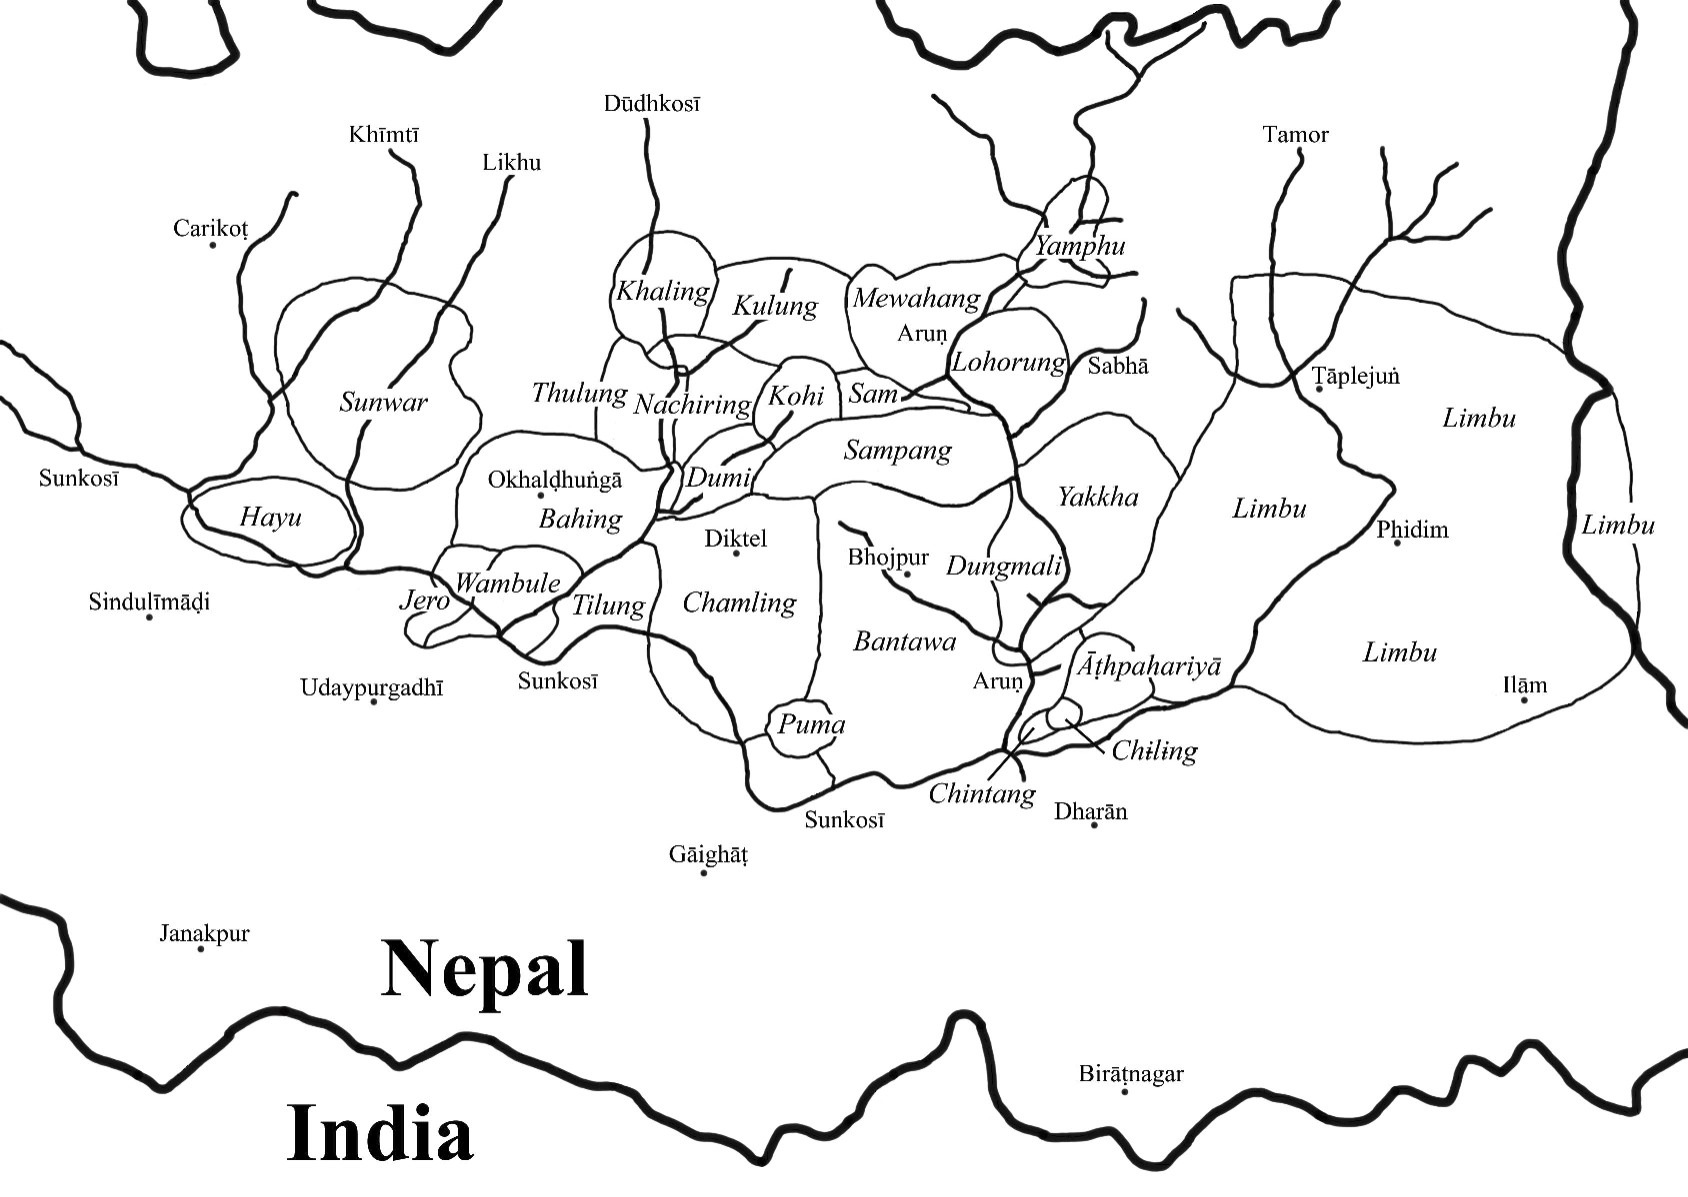
\includegraphics[width=0.7\textwidth]{Kirant.jpeg} \centering
  
  
  \end{frame} 

  \begin{frame} 
 \frametitle{Langues rgyalronguiques (japhug, stau, zbu et khroskyabs)}
  Guillaume \textsc{Jacques}, \textsc{Lai} Yunfan et \textsc{Gong} Xun (CRLAO)
 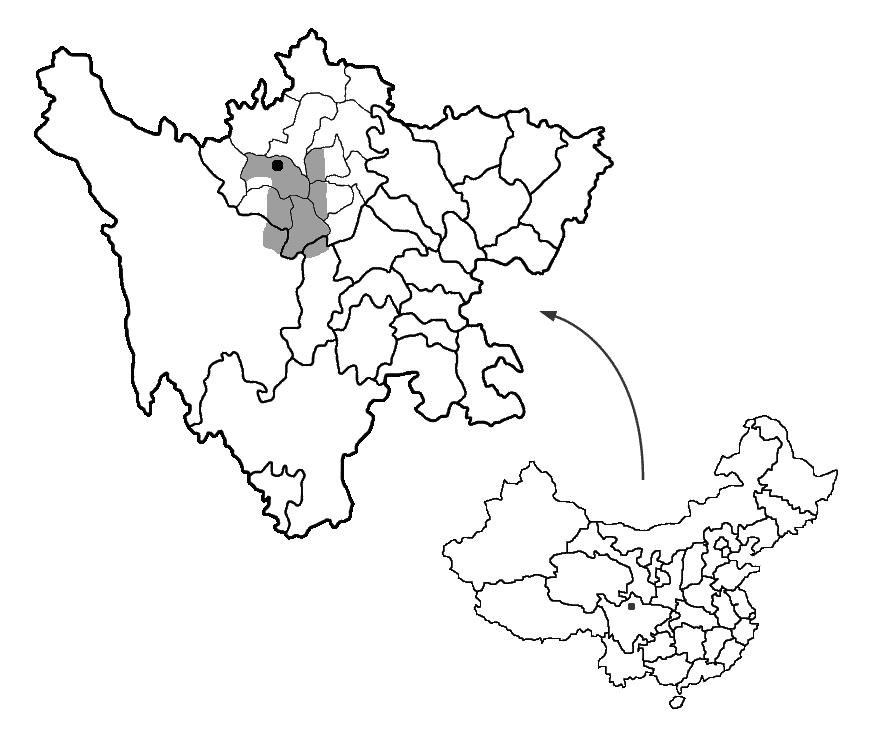
\includegraphics[width=0.6\textwidth]{carte.JPG} \centering
 
  \end{frame}  
 
  \begin{frame} 
 \frametitle{Langues naish (na, naxi)}
 
 Alexis Michaud (MICA/LACITO)
  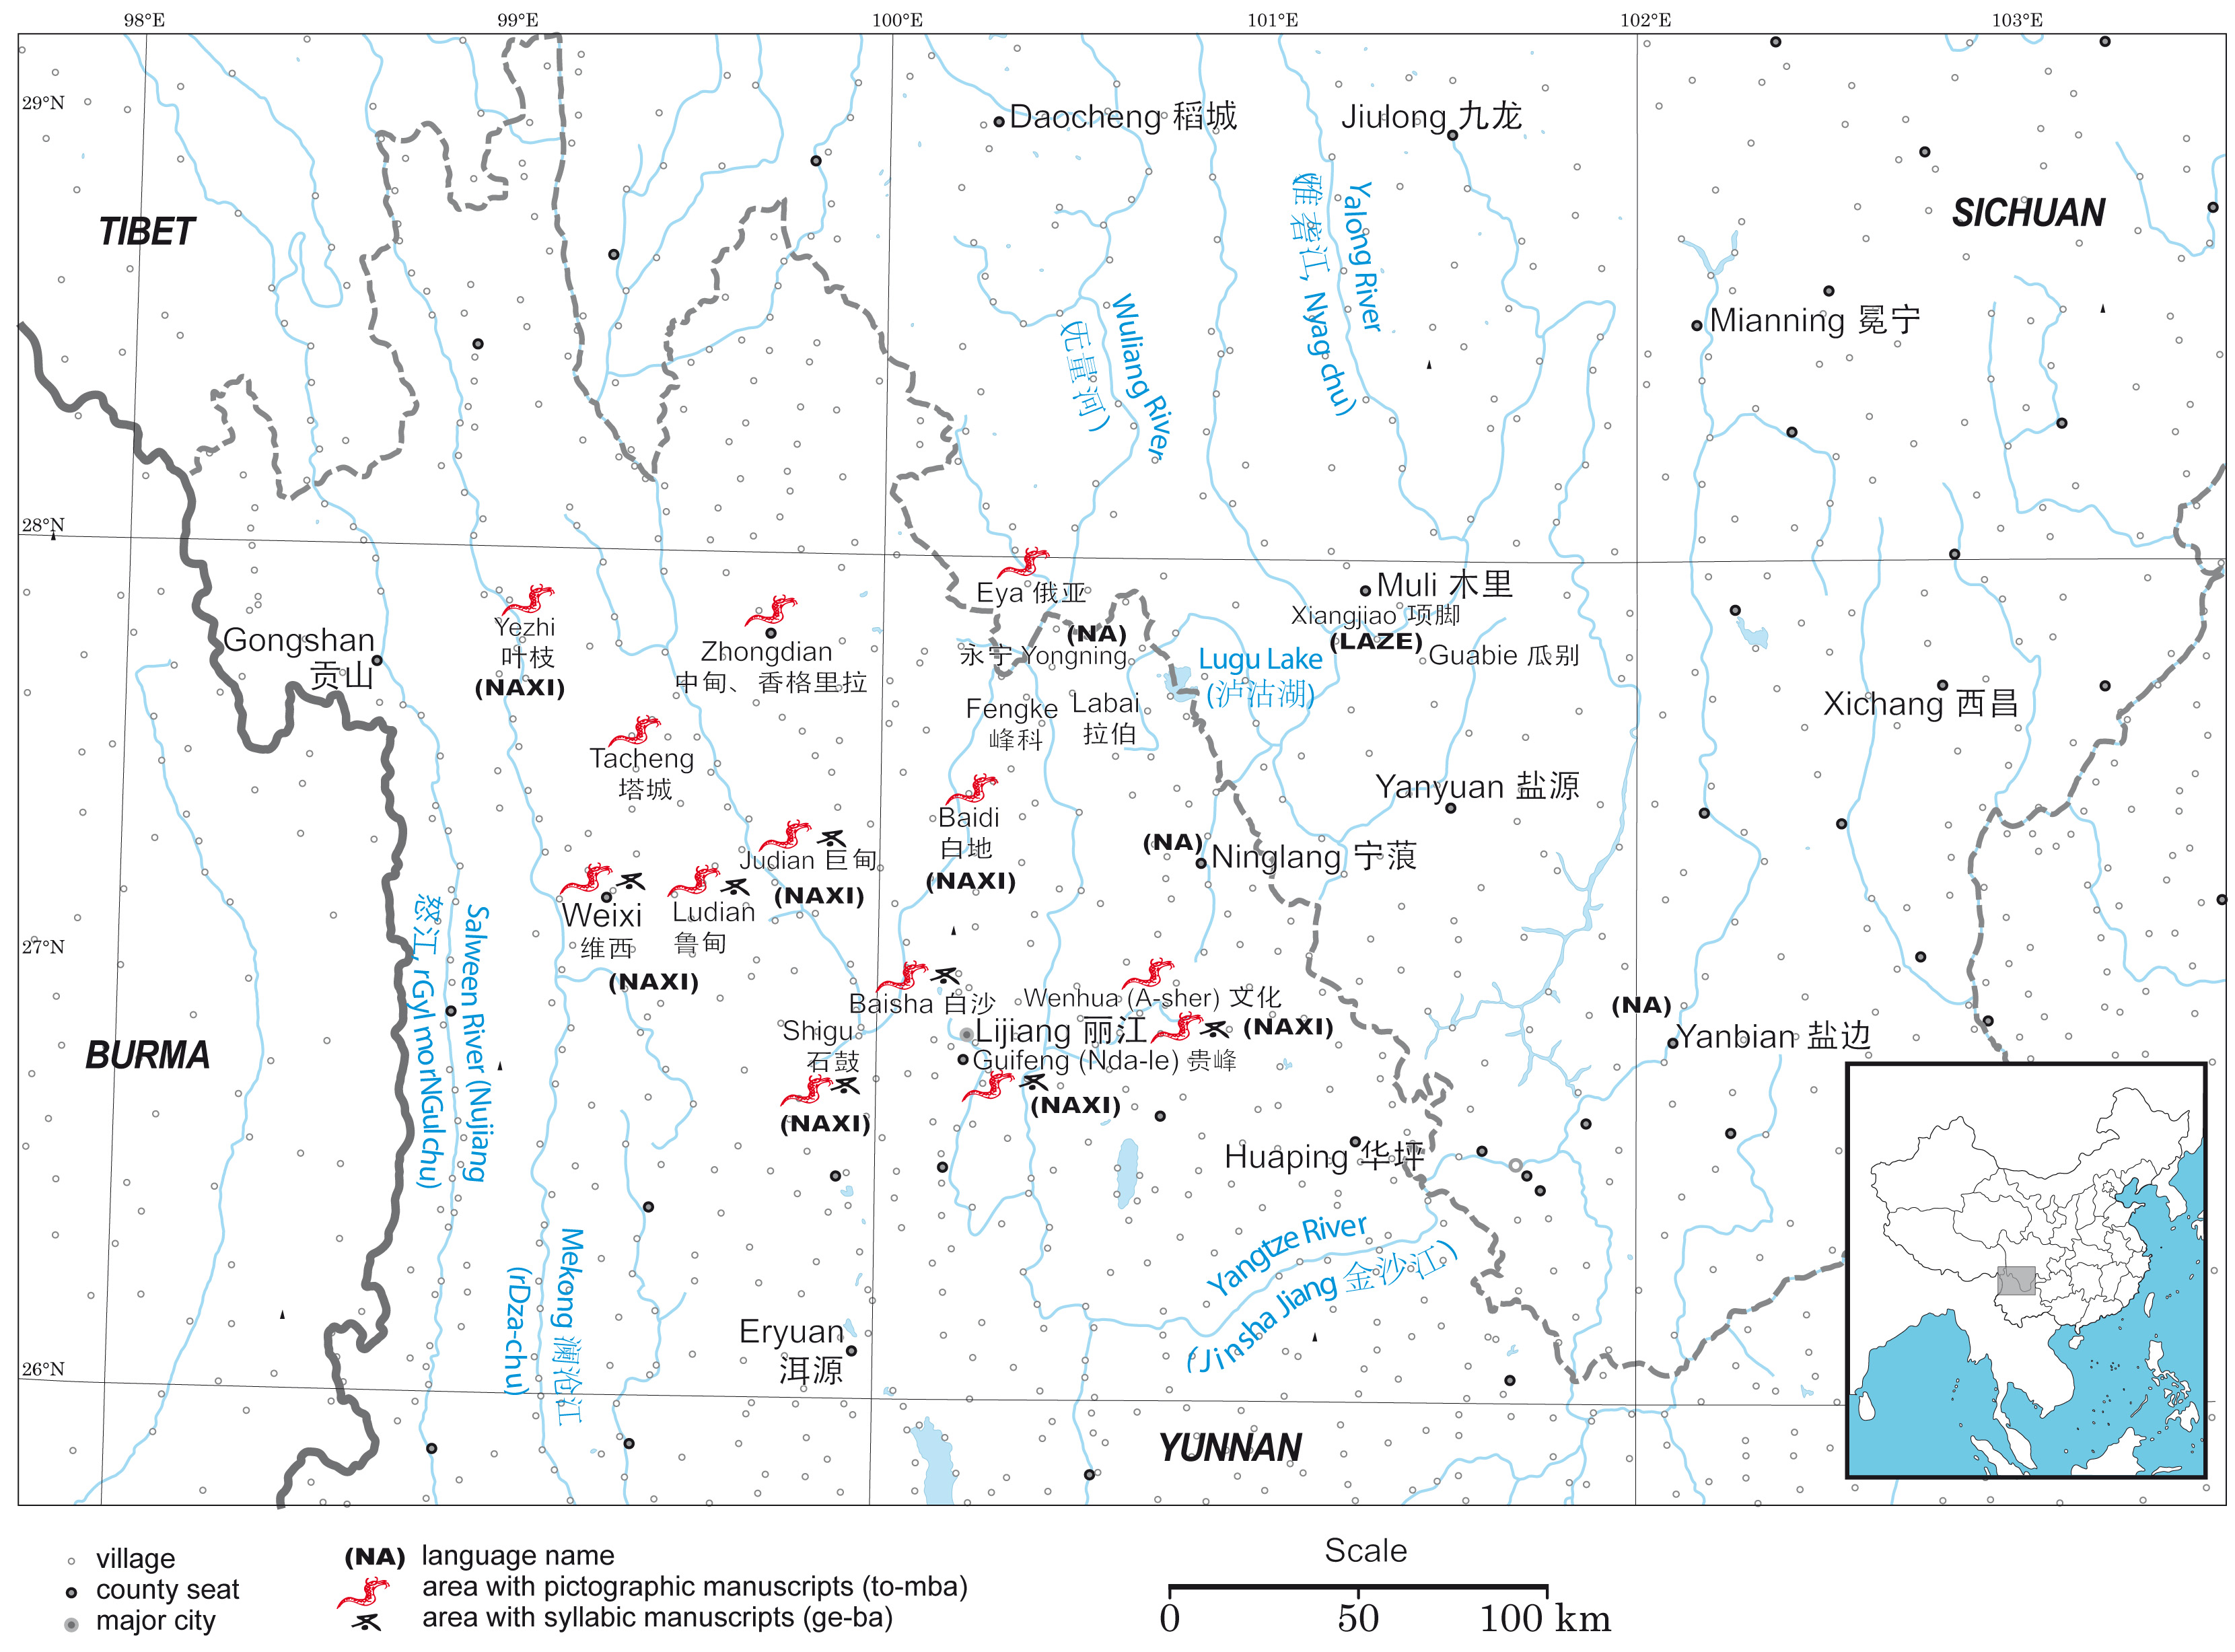
\includegraphics[width=0.9\textwidth]{naish.jpg} \centering
 
  \end{frame}   
 
 \begin{frame} 
 \frametitle{Corpus de textes}

Textes enregistrés et analysés depuis le début du projet (2013)

\begin{enumerate}[<+->]
\item Japhug (19h d'audio, 1h30 de vidéo, dont 8h déjà transcrites)
\item  Na (10h, dont 1h30 traduite)
\item  Khaling (2h, dont une heure traduite)
\item  Thulung (2h transcrites)
\end{enumerate}

 Ces textes seront hébergés à la fin du projet sur l'archive en ligne Pangloss \bleu{http://lacito.vjf.cnrs.fr/pangloss/}
 \end{frame} 
 
 
  \begin{frame} 
 \frametitle{Dictionnaires avec ressources sonores}
 
\begin{enumerate}[<+->]
\item Dictionnaire japhug-chinois-français (environ 700pp, 6245 entrées)
\item  Dictionnaire des verbes khaling-népali-anglais (148pp, 653 entrées)
\item  Dictionnaire na (environ 400pp, 2986 entrées)
\end{enumerate}
 
  \end{frame}    
 
  \begin{frame} 
 \frametitle{Logiciels (1)}
 
\begin{enumerate}[<+->]
\item Recrutement de Céline Buret (ingénieur informaticienne de nov. 2013 à nov. 2015)
\item  Librairie python pour implémenter le format LMF (en cours)
\begin{itemize}
\item Outils de conversion du format MDF (Toolbox) vers un format XML basé sur LMF
\item Conversion LMF $\rightarrow$ HTML / \LaTeX / RTF
\item La librairie python servira pour un projet de programme de conception de dictionnaires et de parsage morphologique dans le cadre du Labex EFL.
\item Documentation et diffusion de cette librairie (article en préparation).
\end{itemize}
\end{enumerate}
  \end{frame}    
  
  \begin{frame} 
 \frametitle{Logiciels (2)}
 
\begin{enumerate}[<+->]
\item Scripts en PERL ou en Python pour répondre à des problèmes spécifiques (programme permettant de renommer automatiquement les fichiers, convertisseurs entre formats d'archivage)
\item Plateforme en ligne de textes parallèles
\item Développement d'une interface android pour les dictionnaires et les textes en ligne.
\item Archivage des données sonores liées aux dictionnaires (Nakala)
\item Création d'un site web pour le projet HimalCo (HumaNum)
\item Générateurs de paradigmes.
\end{enumerate}
 
  \end{frame}     
 
  \begin{frame} 
 \frametitle{Publications}
  \framesubtitle{Articles (2013-2014)}
     \bibliographystyle{Linquiry2}
  \nobibliography{bibliogj.bib}
  \tiny
    \begin{enumerate}
\item  \bibentry{jacques13tropative}
\item {\bibentry{jacques13harmonization}}
\item {\bibentry{lai13fuyin}}
\item {\bibentry{michaud13numeral}}
\item {\bibentry{michailovsky14pangloss}}
\item {\bibentry{antonov14need}}
\item {\bibentry{japhug14ideophones}}
\item {\bibentry{jacques14antipassive}}
\item {\bibentry{jacques14auditory}}
\item {\bibentry{jacques14inverse}}
\item {\bibentry{jacques14linking}}
\end{enumerate}
  \end{frame}      
  
  
    \begin{frame} 
 \frametitle{Publications}
  \framesubtitle{Présentations à des conférences (2013-2014)}
  \tiny
    \begin{enumerate}
\item {\bibentry{jacques13derivational.khaling}}
\item {\bibentry{michaud13leveltone}}
\item {\bibentry{gong14prosodic.tibetan}}
\item {\bibentry{gong14prenasalized}}
\item {\bibentry{do14automatic.processing.na}}
\item  {\bibentry{walther14inv.canon}}
\item {\bibentry{walther14compactness}}

 
\end{enumerate}
  \end{frame}      
 
 
\end{document}


